\section{Introduction}
\label{sec:introduction_009}

Accurate and rigorous uncertainty estimation is key for reliable machine learning models in safety-critical domains \cite{interpretable-ml}. It quantifies the confidence of machine learning models, thus allowing them to validate knowledgeable predictions or flag predictions on unknown input domains. Uncertainty is commonly divided in \emph{aleatoric} and \emph{epistemic} uncertainty \cite{Gal2016a}. The aleatoric uncertainty accounts for irreducible uncertainty (e.g., due to inherent sensor noise). The \emph{epistemic} uncertainty accounts for a lack of information for accurate prediction (e.g., test data significantly different from training data).

Traditionally, machine learning models assume i.i.d.\ inputs, thus performing predictions based on input features only. For uncertainty estimation on i.i.d.\ inputs, a large class of definitions, models and evaluation methods have been introduced \citep{Gal2016a, Malinin2017, Abdar2020, Ovadia2019, robustness-uncertainty-dirichlet}. Further, uncertainty estimation has been successfully applied to different tasks e.g. out-of-distribution (OOD) or shift detection \citep{Ovadia2019}, active learning \cite{uncertainty-meta-learning, bayesian-meta-learning}, continual learning \citep{uncertainty-continual-learning} or reinforcement learning \citep{uncertainty-rl}. 

In contrast, uncertainty estimation on interdependent nodes is more complex than on i.i.d.\ inputs and under-explored \citep{Abdar2020}. A node in an attributed graph is characterized by two types of information: its features and its neighborhood. While the feature information indicates the node position in the feature space -- similarly to i.i.d. inputs --, the neighborhood information indicates the additional node position in the network space. To leverage the neighborhood information, recent graph neural networks (GNNs) successfully proposed to enrich and correct the possibly noisy information of the features of a single node by aggregating them with the features of its neighborhood \cite{Kipf2016, Velickovic2017, Klicpera2018}. It naturally leads to the distinction between predictions \emph{without network effects} based exclusively on their own node feature representation, and predictions \emph{with network effects} based on neighborhood aggregation. The aggregation step commonly assumes \emph{network homophily} which states that nodes with similar properties tend to connect to each other more densely, thus violating the i.i.d. assumption between node features given their neighborhood. 

\looseness=-1
The core motivation of our work is to transfer some of the existing uncertainty estimation definitions, models and evaluations from i.i.d. inputs to interdependent node inputs by leveraging both the feature and the neighborhood information. In particular, we aim at an accurate quantification of the aleatoric and epistemic uncertainty without and with network effect under network homophily (see Fig.~\ref{fig:uncertainty_types_small}).

\looseness=-1
\paragraph{Our contribution.} In this work, we consider uncertainty estimation on semi-supervised node classification. First, we derive three axioms which materialize reasonable uncertainty for non-independent inputs. These axioms cover the traditional notions of aleatoric and epistemic uncertainty and distinguish between the uncertainty with and without network effects. Second, we propose \GPN{} (\GPNacro{})\footnote{Project page including code at \url{https://www.daml.in.tum.de/graph-postnet}} for uncertainty estimation for node classification and prove formally that it follows the axiom requirements contrary to popular GNNs. Third, we build an extensive evaluation setup for uncertainty estimation which relies on the assessment of uncertainty estimation quality of OOD detection and robustness against shifts of the attributed graph properties. Both OOD data and attributed graph shifts distinguish between attribute and structure anomalies. The theoretical properties of \GPNacro{} manifest in these experiments where it outperforms all other baselines on uncertainty evaluation.

\begin{figure}
\centering
	\begin{subfigure}[t]{0.24\textwidth}
	    \centering
		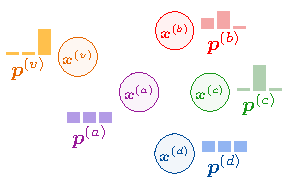
\includegraphics[width=\textwidth]{sections/009_neurips2021/resources/no-network-aleatoric.pdf}
		\caption{AU w/o network}
		\label{subfig:au_without_network}
	\end{subfigure}
	\begin{subfigure}[t]{0.24\textwidth}
	    \centering
		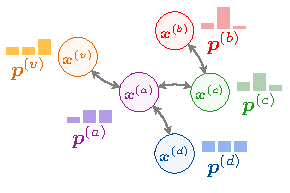
\includegraphics[width=\textwidth]{sections/009_neurips2021/resources/network-aleatoric.pdf}
		\caption{AU w/ network}
		\label{subfig:au_with_network}
	\end{subfigure}
	\begin{subfigure}[t]{0.24\textwidth}
	    \centering
		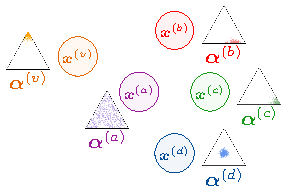
\includegraphics[width=\textwidth]{sections/009_neurips2021/resources/no-network-epistemic.pdf}
		\caption{EU w/o network}
		\label{subfig:eu_without_network}
	\end{subfigure}
	\begin{subfigure}[t]{0.24\textwidth}
	    \centering
		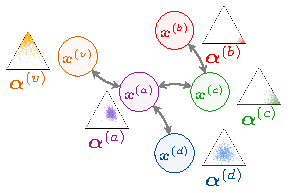
\includegraphics[width=\textwidth]{sections/009_neurips2021/resources/network-epistemic.pdf}
		\caption{EU w/ network}
		\label{subfig:eu_with_network}
	\end{subfigure}
	\caption{Illustration of aleatoric uncertainty (AU) and epistemic uncertainty (EU) without and with network effects (i.e. i.i.d.\ inputs vs interdependent inputs). Nodes have the same features in all cases. Network effects are visualized through edges between nodes which change the predicted distributions. The aleatoric uncertainty is high if the categorical distribution $\hat{\y} \nodeidxv \sim \DCat(\p\nodeidxv)$ is flat. The epistemic uncertainty is high if the Dirichlet distribution $\p\nodeidxv \sim \DDir(\valpha\nodeidxv)$ is spread out. We refer the reader to Section~\ref{subsec:ours} for formal definitions of those distributions.}
    \label{fig:uncertainty_types_small}
\end{figure}
